%\chapterimage{Geometrijska.jpg} % Chapter heading image

\chapter{Svetloba kot elektromagnetno valovanje}
V tem poglavju bomo prešli z geometrijskega  na valovni opis svetlobe in jo 
obravnavali kot elektromagnetno valovanje. Iz Maxwellovih enačb
bomo izpeljali valovno enačbo in poiskali njene rešitve.
Zapisali bomo energijski tok
in vpeljali polarizacijo elektromagnetnega valovanja. Na koncu
bomo zapisali še valovno enačbo v prevodni snovi in vpeljali 
kompleksni lomni količnik. 

\section{Valovna enačba v neprevodni snovi}
Obravnavajmo širjenje svetlobe po homogeni, izotropni in neprevodni snovi, 
v kateri ni prostih nabojev in električnih tokov. Na splošno elektromagnetno polje
opišemo z jakostjo  $\mathbf{E}$ in gostoto električnega polja $\mathbf{D}$
ter gostoto $\mathbf{B}$ in jakostjo magnetnega polja $\mathbf{H}$. Te vektorske
količine med seboj niso neodvisne. Za količine električnega polja velja:
\beq
\mathbf{D} = \varepsilon \varepsilon_0 \mathbf{E},
\label{eq:DE}
\eeq
pri čemer sta $\varepsilon$ dielektričnost (ali tudi električna permitivnost) in $\varepsilon_0$
influenčna konstanta z vrednostjo $\varepsilon_0 = 8,85 \times 10^{-12}~\si{As/Vm}$. 
Med količinami magnetnega polja velja zveza:
\beq
\mathbf{H} = \frac{\mathbf{B}}{\mu \mu_0},
\label{eq:HB}
\eeq
pri čemer je $\mu$ magnetna permeabilnost, konstanta $\mu_0$ pa je 
indukcijska konstanta z vrednostjo $\mu_0 = 4 \pi \times 10^{-7}~\si{Vs/Am}$.
Privzeli smo, da je snov izotropna, sicer bi morali $\varepsilon$ in $\mu$ pisati v 
tenzorski obliki. Prav tako smo privzeli, da so polja v snovi dovolj šibka, da
se snov odziva linearno. Nelinearen odziv, ki ga obravnava obširno področje
nelinearne optike, presega okvir te knjige.\footnote{~Glej npr. M. Čopič in M. Vilfan, 
{\it Fotonika}, Založba FMF, 2020.}

Količine elektičnega in magnetnega polja med seboj povezujejo Maxwellove
enačbe:
\boxeq{eq:Maxwell1}{
\nabla\times\mathbf{H} & =\frac{\partial\mathbf{D}}{\partial t}+\mathbf{j}_e,\\
\nabla\times\mathbf{E} & =-\frac{\partial\mathbf{B}}{\partial t}\label{eq:Maxwell2},\\
\nabla\cdot\mathbf{D} & =\varrho_{e}\label{eq:Maxwell3} \qquad \mathrm{in}\\
\nabla\cdot\mathbf{B} & =0.\label{eq:Maxwell4}
}

Enačbe smo zaradi splošnosti zapisali v celotni obliki. Mi bomo 
obravnavali le primer, ko sta gostota električnega toka $\mathbf{j}_e$ in 
gostota prostih nabojev $\varrho_e$ enaki nič.  

\begin{remark}
Prvo od zapisanih Maxwellovih enačb imenujemo tudi Amp\`{e}rov zakon,
drugo Faradayev indukcijski zakon,
tretjo Gaussov zakon in četrto po analogiji Gaussov zakon za magnetno polje.
\end{remark}

Izhajamo iz enačbe~(\ref{eq:Maxwell2}) in na njej naredimo rotor:
\beq
\nabla \times \left(\nabla\times\mathbf{E}\right) =
\nabla \times \left(-\frac{\partial \mathbf{B}}{\partial t} \right)\!\!.
\label{eq:03_01}
\eeq
Levo stran enačbe preoblikujemo z upoštevanjem splošne zveze:
\beq
\nabla \times (\nabla \times \mathbf{E}) = \nabla (\nabla \cdot \mathbf{E}) - \nabla^2 \mathbf{E}.
\label{eq:03_02}
\eeq
Poglejmo prvi člen podrobneje. Jakost električnega polja $\mathbf{E}$ najprej  
izrazimo z $\mathbf{D}$ (enačba~\ref{eq:DE}), nato pa upoštevmo še Gaussov zakon 
(enačba~\ref{eq:Maxwell3}). Sledi:
\beq
\nabla \times (\nabla \times \mathbf{E}) = \nabla \left(\nabla \cdot 
\frac{\mathbf{D}}{\varepsilon \varepsilon_0}\right) - \nabla^2 \mathbf{E} = - \nabla^2 \mathbf{E}.
\label{eq:03_03}
\eeq
Na desni strani enačbe~(\ref{eq:03_01}) odvoda po kraju in času zamenjamo, 
saj sta neodvisna. Upoštevamo enačbo~(\ref{eq:HB}) in Amp\`{e}rov zakon (enačba~\ref{eq:Maxwell1}). Dobimo:
\beq
\nabla \times \left(-\frac{\partial \mathbf{B}}{\partial t} \right) = 
- \frac{\partial}{\partial t}\left(\mu \mu_0 \nabla
\times \mathbf{H}\right) = - \mu \mu_0 \frac{\partial}{\partial t}\frac{\partial \mathbf{D}}{\partial t}.
\label{eq:03_04}
\eeq
Izrazimo še gostoto električnega polja z jakostjo (enačba~\ref{eq:DE}) in izraz izenačimo z 
izračunano levo stranjo enačbe (enačba~\ref{eq:03_03}). Dobimo valovno enačbo:
\boxeq{eq:valovnaE}{
\nabla^2\mathbf{E} - \varepsilon \varepsilon_0 \mu \mu_0 \frac{\partial^2 \mathbf{E}}{\partial t^2} = 0.
}
Ponovimo še zapis leve strani valovne enačbe s komponentami:
\beq
\nabla^2 \mathbf{E} =  
\left[\begin{array}{c}
        \frac{\partial^2E_x}{\partial x^2} + \frac{\partial^2E_x}{\partial y^2} + \frac{\partial^2E_x}{\partial z^2}\\
        \frac{\partial^2E_y}{\partial x^2} + \frac{\partial^2E_y}{\partial y^2} + \frac{\partial^2E_y}{\partial z^2} \\
        \frac{\partial^2E_z}{\partial x^2} + \frac{\partial^2E_z}{\partial y^2} + \frac{\partial^2E_z}{\partial z^2}
      \end{array}\right]\!\!.
\label{eq:03_05}
\eeq
Valovno enačbo lahko izpeljemo tudi za gostoto magnetnega polja:
\begin{equation}
\nabla^2\mathbf{B} - \varepsilon \varepsilon_0 \mu \mu_0 \frac{\partial^2 \mathbf{B}}{\partial t^2} = 0.
\label{eq:valovnaB}
\end{equation}
V nadaljevanju bo naša naloga poiskati rešitve teh dveh valovnih enačb $\mathbf{E(\mathbf{r},t)}$
in $\mathbf{B(\mathbf{r},t)}$ kot funkciji kraja $\mathbf{r}$ in časa $t$ pri danih robih pogojih.

\section{Ravni valovi}
Najpreprostejša rešitev valovne enačbe je sinusno potujoče valovanje, ki ga zapišemo
v obliki:
\boxeq{eq:ravnival}{
\mathbf{E}(\mathbf{r},t) = \mathbf{E}_0 \cos \left(\mathbf{k}\cdot \mathbf{r} - \omega t + \delta\right) = 
\Re\left(\mathbf{E}_0 e^{i\mathbf{k}\cdot \mathbf{r} - i\omega t + i\delta}\right)
}
in 
\beq
\mathbf{B}(\mathbf{r},t) = \mathbf{B}_0 \cos \left(\mathbf{k}\cdot \mathbf{r} - \omega t + \delta\right) = 
\Re\left(\mathbf{B}_0 e^{i\mathbf{k}\cdot \mathbf{r} - i\omega t + i\delta}\right)\!\!.
\label{eq:ravnivalB}
\eeq
Pri tem nastavku sta amplitudi valovanja $\mathbf{E}_0$ in $\mathbf{B}_0$ konstantni, 
$\mathbf{k}$ označuje valovni vektor, 
$\omega$ krožno frekvenco in $\delta$ konstantno fazo
valovanja. 

Potujoče sinusno valovanje, kakršnega opisuje enačba~(\ref{eq:ravnival}), preprosto
narišemo, pri čemer se zaradi nazornosti omejimo na valovanje, ki potuje v smeri $z$. 
Ob danem trenutku (pri izbranem $t$) je odvisnost električnega polja od
koordinate prikazana na sliki~\ref{fig:03_sinus}. Podobno lahko narišemo tudi 
sinusno odvisnost od časa na danem mestu (pri izbranem $z$). 

\begin{figure}[!h]
\centering
\def\svgwidth{90truemm} 
\input{slike/03_sinus.pdf_tex}
\caption{Jakost električnega polja kot sinusno potujoče valovanje ob nekem izbranem času.}
\label{fig:03_sinus}
\end{figure}

Iz slike razberemo
zvezo $k\lambda = 2\pi$, ki jo uporabimo za izračun velikosti valovnega
vektorja:
\boxeq{eq:valovnivektor}{
k = \frac{2\pi}{\lambda}.
}
Vrnimo se k nastavku in celotno fazo, torej argument kotne funkcije, označimo s $\phi$:
\beq
\phi = \mathbf{k}\cdot \mathbf{r} - \omega t + \delta.
\label{eq:03_06}
\eeq
Ploskve konstantne faze dobimo pri konstantnem $\phi$. Ob danem trenutku velja:
\beq
\mathbf{k}\cdot \mathbf{r} = \phi + \omega t - \delta = \mathrm{konst.}
\label{eq:03_08}
\eeq
Ta pogoj ni nič drugega kot enačba ravnine, pravokotne na vektor $\mathbf{k}$. Ploskve konstantne faze
oziroma valovne fronte so torej ravnine, ki so pravokotne na $\mathbf{k}$, žarki pa so premice, ki 
so vzporedne s $\mathbf{k}$. Zapisana rešitev predstavlja ravni val.
\begin{figure}[ht]
\centering
\def\svgwidth{90truemm} 
\input{slike/03_ravnival.pdf_tex}
\caption{Najpreprostejša rešitev valovne enačbe je ravni val, pri katerem so ploskve konstante
faze (valovne fronte) ravnine, pravokotne na valovni vektor $\mathbf{k}$.}
\label{fig:03_ravnival}
\end{figure}
\begin{remark}
Jakost elektičnega polja je realna količina, kar je razvidno tudi iz zapisa (enačba~\ref{eq:ravnival}). 
V računih pogosto uporabljamo kompleksni zapis, to je brez omejitve na realni del. To lahko 
naredimo, dokler so jakosti polja majhne in velja linearna optika. Račun s kompleksnim zapisom
je navadno precej preglednejši in preprostejši, vendar moramo na koncu računa vedno vzeti le
realni del izračunane jakosti električnega polja. 
\end{remark}

\subsection*{Fazna hitrost}
Fazna hitrost je hitrost premikanja ploskev konstantne faze oziroma valovnih front. 
Če sledimo valovni ploskvi, je odvod faze po času konstanten in iz enačbe~(\ref{eq:03_06}) 
dobimo:
\beq
\frac{d\phi}{dt}= \mathbf{k}\cdot \frac{d\mathbf{r}}{dt} - \omega = 0.
\label{eq:03_09}
\eeq
Zanima nas potovanje v smeri vzdolž $\mathbf{k}$, 
zato lahko zapišemo $\mathbf{k}\cdot \mathbf{r} = kr$. Hitrost premikanja ploskev
konstantne faze oziroma fazna hitrost je potem enaka:
\beq
v_f = \frac{dr}{dt} = \frac{\omega}{k}.
\label{eq:03_10}
\eeq
Pri tem je $k$ velikost valovnega vektorja, ki jo imenujemo valovno število.
Poiščimo zvezo med $\omega$ in $k$ in izračunajmo fazno hitrost.

Nastavek 
(enačba~\ref{eq:ravnival}) vstavimo v valovno enačbo (enačba~\ref{eq:valovnaE}). 
Obravnavajmo zaenkrat samo eno komponento, na koncu razširimo zapis na tri komponente. 
Za komponento v smeri $x$ dobimo:
\begin{align}
\nabla^2E_x =& \frac{\partial^2E_x}{\partial x^2} + \frac{\partial^2E_x}{\partial y^2} + 
\frac{\partial^2E_x}{\partial z^2} \nonumber \\
=& \left(\frac{\partial^2}{\partial x^2} + 
\frac{\partial^2}{\partial y^2} + \frac{\partial^2}{\partial z^2}\right) \left(
E_{0x} \exp\left( ik_xx+ik_yy+ik_zz -i\omega t + \delta\right) \right)\nonumber \\
=& \left( -k_x^2 -k_y^2-k_z^2\right) E_{0x} \exp\left( ik_xx+ik_yy+ik_zz -i\omega t + \delta\right)\nonumber \\
=& -k^2 E_{0x} \exp\left( ik_xx+ik_yy+ik_zz -i\omega t + \delta\right) = -k^2 E_x.
\label{eq:03_11}
\end{align}
Podoben izračun naredimo še za ostali komponenti in združeno zapišemo:
\beq
\nabla^2\mathbf{E}= -k^2 \mathbf{E}.
\label{eq:03_12}
\eeq
Odvajajmo nastavek (enačba~\ref{eq:ravnival}) še dvakrat po času:
\beq
\frac{\partial^2 \mathbf{E}}{\partial t^2} = - \omega^2 \mathbf{E}.
\label{eq:03_13}
\eeq
Iz valovne enačbe tako dobimo zvezo:
\beq
-k^2 \mathbf{E} + \varepsilon\varepsilon_0\mu\mu_0 \omega^2 \mathbf{E} = 0
\quad \Longrightarrow \quad
k = \sqrt{\varepsilon\varepsilon_0\mu\mu_0}\,\omega.
\label{eq:03_15}
\eeq
Zdaj lahko zapišemo fazno hitrost:
\beq
v_f = \frac{\omega}{k} = \frac{1}{\sqrt{\varepsilon_0\mu_0}}\frac{1}{\sqrt{\varepsilon\mu}}.
\label{eq:fazna}
\eeq
Kadar se elektromagnetno valovanje širi v praznem prostoru, sta $\varepsilon = 1$ in $\mu=1$. 
Označimo s $c_0$ hitrost elektromagnetnega valovanja -- in s tem tudi svetlobe -- v praznem prostoru:
\boxeq{eq:c0}{
c_0 = \frac{1}{\sqrt{\varepsilon_0\mu_0}}.
}
V snovi je fazna hitrost potovanja svetlobe, ki jo navadno označujemo s $c$, manjša, in sicer:
\beq
c = v_f = \frac{c_0}{\sqrt{\varepsilon\mu}} = \frac{c_0}{n}.
\label{eq:03_16}
\eeq
Pri tem smo vpeljali lomni količnik snovi $n = \sqrt{\varepsilon\mu}$. 
V optiki večinoma obravnavamo snovi, ki niso magnetne, zato je lomni količnik kar
enak korenu iz dielektričnosti:
\boxeq{eq:n}{
n = \sqrt{\varepsilon}.
}
\vglue-3truemm
\begin{remark}
Ne smemo pozabiti, da se dielektričnost s frekvenco elektromagnetnega 
valovanja spreminja. Pri izračunu lomnega količnika moramo zato upoštevati vrednost
dielektričnosti pri krožni frekvenci vidne svetlobe, kar je $\omega \sim 3 \times 10^{15}~\si{s}^{-1}$. 
\end{remark}

% \begin{table}[ht]
%  \centering
%  \small
% \begin{tabular}{|l|c||l|c|} \hline  
%       Snov & $n$ & Snov & $n$ \\ \hline
%       zrak & 1,00027 & glicerol & 1,47\\ \hline
%       voda & 1,33 & steklo & 1,4 -- 1,9\\ \hline 
%       led & 1,31 & safir & 1,77\\ \hline
%       etanol & 1,36 & diamant & 2,42\\ 
% \hline 
% \end{tabular}
%   \caption{Lomni količniki nekaterih izbranih snovi}
% \label{table:n}
% \end{table}

Vrnimo se k hitrosti svetlobe. Z upoštevanjem enačbe~(\ref{eq:valovnivektor})
izraz za $c$ preoblikujemo:
\begin{equation}
 c = \frac{\omega}{k} = \frac{2 \pi \nu}{2 \pi/\lambda},
 \label{eq:03_17}
\end{equation}
pri čemer smo vpeljali frekvenco $\nu = \omega/2\pi$. 
Sledi:
\boxeq{eq:nulambda}{
c = \nu \lambda.
}
Produkt frekvence in valovne dolžine je torej enak fazni hitrosti svetlobe. Ker 
se v snovi hitrost svetlobe zmanjša, hkrati pa frekvenca ohranja, se torej 
v snovi zmanjša valovna dolžina valovanja. Če je v praznem prostoru valovna dolžina
$\lambda_0$, potem je v snovi z lomnim količnikom $n$ valovna dolžina enaka:
\beq
\lambda = \frac{\lambda_0}{n}.
\label{eq:03_18}
\eeq

\subsection*{Smeri vektorjev $\mathbf{E}$, $\mathbf{B}$ in $\mathbf{k}$}
Nadaljujmo z obravnavo elektromagnetnega valovanja v homogeni in izotropni snovi. 
Valovanje naj bo v obliki ravnih valov, pri čemer se poslužimo praktičnega kompleksnega zapisa:
\beq
\mathbf{E}(\mathbf{r},t) = \mathbf{E}_0 e^{i\mathbf{k}\cdot \mathbf{r} - i\omega t + i\delta}
\qquad \mathrm{in} \qquad
\mathbf{B}(\mathbf{r},t) = \mathbf{B}_0 e^{i\mathbf{k}\cdot \mathbf{r} - i\omega t + i\delta}.
\label{eq:ravnivalkompleks}
\eeq
Izhajamo iz Gaussovega zakona (enačba~\ref{eq:Maxwell3}) in upoštevamo zvezo med 
$\mathbf{D}$ in $\mathbf{E}$ (enačba~\ref{eq:DE}): 
\beq
\nabla \cdot \mathbf{D} = \nabla \cdot \left( \varepsilon \varepsilon_0 \mathbf{E}\right) 
= \varepsilon \varepsilon_0 \left(\nabla \cdot \mathbf{E} \right).
\label{eq:03_20}
\eeq
Iz tega sledi, da je ob odsotnosti prostih nabojev ($\varrho_{e} = 0$) divergenca 
jakosti električnega polja v izotropni snovi enaka nič.
Zapišemo jo kot:
\begin{align}
\nabla \cdot \mathbf{E} = \frac{\partial E_x}{\partial x}+ \frac{\partial E_y}{\partial y}+
\frac{\partial E_z}{\partial z} =& \left(ik_xE_{0x} + ik_yE_{0y} + ik_zE_{0z}\right)
e^{i\mathbf{k}\cdot \mathbf{r} - i\omega t + i\delta}\nonumber\\
=& i \left( \mathbf{E}_0 \cdot \mathbf{k} \right) e^{i\mathbf{k}\cdot \mathbf{r} - i\omega t + i\delta} = 
i\, \mathbf{E} \cdot \mathbf{k} = 0.
\label{eq:03_21}
\end{align}
Pogoj, da je skalarni produkt jakosti električnega polja in valovnega vektorja enak nič, 
je izpolnjen, kadar je:
\boxeq{eq:Ekperp}{
\mathbf{E} \perp \mathbf{k}.
}
Na enak način iz enačbe~(\ref{eq:Maxwell4}) izpeljemo zvezo:
\boxeq{eq:Bkperp}{
\mathbf{B}\perp \mathbf{k}.
}
Elektromagnetno valovanje je torej v izotropni snovi transverzalno, saj sta jakost
električnega in gostota magnetnega polja pravokotni na smer širjenja svetlobe.

Poiščimo še kot med $\mathbf{E}$ in $\mathbf{B}$. Spet izhajamo iz Maxwellove 
enačbe, tokrat iz Faradayevega zakona (enačba~\ref{eq:Maxwell2}). Magnetno polje odvajamo po 
času in dobimo zvezo:
\beq
\nabla\times\mathbf{E} = i \omega \mathbf{B}.
\label{eq:03_22}
\eeq
Nato izračunamo rotor jakosti električnega polja:
\beq
\nabla \times \mathbf{E} = 
\left|
\begin{array}{ccc}
\mathbf{i} & \mathbf{j} & \mathbf{k}\\
\frac{\partial}{\partial x} & \frac{\partial}{\partial y} & \frac{\partial}{\partial z}\\
E_{x} & E_{y} & E_{z}
\end{array}\right|
= 
\left[
\begin{array}{c}
ik_y E_z-ik_zE_y\\
ik_z E_x-ik_xE_z\\
ik_x E_y-ik_yE_x
\end{array}\right] = 
i\, \mathbf{k}\times \mathbf{E}.
\label{eq:03_23}
\eeq
Rezultat vstavimo v enačbo~(\ref{eq:03_22}) in dobimo:
\beq
\mathbf{k}\times \mathbf{E} = \omega \mathbf{B}.
\label{eq:EkB}
\eeq
Sledi, ortogonalnost jakosti električnega $\mathbf{E}$ in gostote magnetnega
polja $\mathbf{B}$:
\boxeq{eq:EBort}{
\mathbf{B}\perp \mathbf{E}.
}
S tem smo pokazali, da so v elektromagntnem valovanju v izotropni snovi
vsi trije vektorji $\mathbf{E}$, $\mathbf{B}$ in $\mathbf{k}$
med seboj paroma pravokotni. Navadno velja dogovor, da je 
$\mathbf{E}\parallel x$, $\mathbf{B}\parallel y$ in $\mathbf{k}\parallel z$.
\begin{figure}[ht]
\centering
\def\svgwidth{120truemm} 
\input{slike/03_orto.pdf_tex}
\caption{Elektromagnetno valovanje v izotropni snovi je transverzalno.}
\label{fig:03_orto}
\end{figure}

\subsection*{Razmerje med $\mathbf{E}_0$ in $\mathbf{B}_0$}
Zdaj poznamo smeri vektorjev $\mathbf{E}$ in $\mathbf{B}$ v ravnem valu, poiskati moramo
še razmerja med njunimi amplitudami. Izhajamo iz enačbe~(\ref{eq:EkB}), upoštevamo
medsebojno pravokotnost vektorjev, pokrajšamo časovno-krajevni del v eksponentu
in dobimo zvezo med amplitudami:
\beq
k E_0 = \omega B_0 \quad \Longrightarrow \quad E_0 = B_0 \frac{\omega}{k}.
\label{eq:03_24}
\eeq
Sledi:
\boxeq{eq:EBc}{
E_0 = B_0c = B_0 \frac{c_0}{n}.
}
Magnetna polja v elektromagnetnem valovanju so zato razmeroma šibka. Na primer vrednosti 
$E_0 = 100~\si{V/m}$ ustreza $B_0 = 0,3~\si{\micro \tesla}$, kar je približno 
stokrat manj kot Zemljino magnetno polje. 

Pogosto nas zanima razmerje med $E_0$ in $H_0$. To razmerje imenujemo impedanca
snovi in jo označimo z $Z$. Enaka je:
\beq
Z = \frac{E_0}{H_0} = \frac{E_0 \mu \mu_0}{B_0} = \mu \mu_0 c = 
\frac{\mu \mu_0}{\sqrt{\varepsilon \varepsilon_0 \mu \mu_0}} = \sqrt{\frac{\mu \mu_0}{\varepsilon \varepsilon_0}}.
\label{eq:03_25}
\eeq
Enote za impedanco so:
\beq
\sqrt{\frac{\si{Vs/Am}}{\si{As/Vm}}} = \frac{\si{V}}{\si{A}} = \si{\ohm}.
\label{eq:03_26}
\eeq
V vakuumu, kjer sta $\varepsilon = 1$ in $\mu= 1$, je impedanca $Z_v = 377~\si{\ohm}$.

\begin{remark}
Poleg ravnih valov, ki predstavljajo enodimenzionalno rešitev valovne enačbe, poznamo
tudi druge rešitve, na primer sferične ali cilindrične valove. Pri sferičnih so ploskve
konstantne faze krogelne lupine, ki izhajajo radialno simetrično iz točke. V tem 
primeru amplituda valovanja ni konstantna, ampak se zmanjšuje z oddaljenostjo 
od izhodišča kot $A = E_0/r$. V primeru cilindričnih valov so ploskve konstatne
faze valji, ki izhajajo iz izhodiščne premice. Tudi v tem primeru se amplituda
z oddaljenostjo od izhodiščne premice spreminja: $A = E_0/\sqrt{r}$.  Če cilindrični 
primer omejimo na eno ravnino (kar zaradi translacijske simetrije lahko naredimo), 
dobimo rešitev dvodimenzionalne valovne enačbe v polarnih koordinatah. 
\begin{figure}[ht]
\centering
\def\svgwidth{120truemm} 
\input{slike/03_sfericnival.pdf_tex}
\caption{Valovne fronte sferičnega vala so krogelne lupine (a), valovne fronte
cilindričnega vala pa valji (b).}
\label{fig:03_sfericnival}
\end{figure}
\end{remark}

\section{Poyntingov vektor in energijski tok}
Pomembna lastnost elektromagnetnega valovanja je prenos energije. V električnem
polju gostoto energije zapišemo kot:\footnote{Glej npr. J. Strnad, {\it Fizika, drugi del}, 
DMFA-založništvo (2018).}
\beq
w_E = \frac{1}{2}\varepsilon \varepsilon_0 \mathbf{E}^2
\label{eq:03_27}
\eeq
in v magnetnem polju kot: 
\beq
w_B = \frac{1}{2\mu \mu_0} \mathbf{B}^2.
\label{eq:03_28}
\eeq
Celotna gostota energije v prostoru je vsota obeh prispevkov:
\beq
w_{EMV} = w_E + w_B = \frac{1}{2}\varepsilon \varepsilon_0 \mathbf{E}^2 + \frac{1}{2\mu \mu_0} \mathbf{B}^2.
\label{eq:03_29}
\eeq
Vstavimo jakost električnega (enačba~\ref{eq:ravnival}) in gostoto magnetnega polja
(enačba~\ref{eq:ravnivalB}). Sledi:
\beq
w_{EMV} = \frac{1}{2}\varepsilon \varepsilon_0 \mathbf{E}_0^2 
\cos^2 \left(\mathbf{k}\cdot \mathbf{r} - \omega t + \delta\right)
+ \frac{1}{2\mu \mu_0} \mathbf{B}_0^2 \cos^2 \left(\mathbf{k}\cdot \mathbf{r} - \omega t + \delta\right).
\label{eq:03_30}
\eeq
Upoštevamo zvezo med amplitudama (enačba~\ref{eq:EBc}) in dobimo:
\beq
w_{EMV} = \left(\frac{1}{2}\varepsilon \varepsilon_0 E_0^2 + 
\frac{1}{2\mu \mu_0} \frac{E_0^2}{c^2} \right) 
\cos^2 \left(\mathbf{k}\cdot \mathbf{r} - \omega t + \delta\right).
\label{eq:03_31}
\eeq
Vstavimo še izraz za hitrost valovanja (enačba~\ref{eq:fazna}) in vidimo,
da sta prispevka električnega in magnetnega polja k gostoti energije po velikosti 
enaka, poleg tega imata enako krajevno in časovno odvisnost:
\beq
w_{EMV} = \left(\varepsilon \varepsilon_0 E_0^2  \right) 
\cos^2 \left(\mathbf{k}\cdot \mathbf{r} - \omega t + \delta\right).
\label{eq:03_32}
\eeq

Za vidno svetlobo je krožna frekvenca zelo velika 
($\omega \sim 3 \times 10^{15}~\si{s}^{-1}$), zato praktično vedno 
zaznavamo povprečno energijo, ki je povprečena po času čez veliko 
število nihanj. Ker je po dolgem času povprečje funkcije $\cos^2(x) = 1/2$, sledi:
\boxeq{eq:w}{
\langle w \rangle = \frac{1}{2}\varepsilon \varepsilon_0 E_0^2. 
}
Gostota energijskega ali svetlobnega toka dobimo tako, da gostoto energije
pomnožimo s hitrostjo valovanja $c$. Čeprav gre za časovno povprečje gostote
toka, ga navadno označujemo samo z $j$:
\boxeq{eq:j}{
j = \langle w \rangle c = \frac{1}{2}\varepsilon \varepsilon_0 E_0^2 c.
}

\begin{remark}
V snoveh, za katere velja $\mu = 1$, je $n = \sqrt{\varepsilon}$. Potem izraz za gostoto
energijskega toka zapišemo kot:
\beq
j = \frac{1}{2}\varepsilon \varepsilon_0 E_0^2 \frac{c_0}{\sqrt{\varepsilon}} = 
\frac{1}{2}\sqrt{\varepsilon} \varepsilon_0 E_0^2 c_0 = \frac{1}{2} \varepsilon_0 E_0^2 c_0 n.
\label{eq:03_33}
\eeq
\end{remark}

V izotropnih snoveh se energijski tok širi v smeri žarkov in lahko zapišemo 
$\mathbf{j}\parallel \mathbf{k}$. Splošnejši izraz, ki velja tudi v anizotropnih snoveh, je
zapis s Poyntingovim vektorjem $\mathbf{S}$. Vpeljemo ga kot:
\boxeq{eq:Poyntingov}{
\mathbf{S} = \mathbf{E}\times\mathbf{H}.
}

Preverimo, da je v izotropni snovi $\mathbf{S} = \mathbf{j}$, kot smo ga zapisali 
v enačbi~(\ref{eq:j}). Vpeljemo najprej vektor $\mathbf{s}$, ki je enotski vektor
v smeri valovnega vektorja, in predstavlja smer potovanja energije:
\beq
\mathbf{s} = \frac{\mathbf{k}}{k}.
\label{eq:03_34}
\eeq
Zapišemo:
\begin{align}
\mathbf{S}= &\, \mathbf{E}\times \mathbf{H} = \left( \mathbf{E}_0\times \mathbf{H}_0 \right)
\cos^2 \left(\mathbf{k}\cdot \mathbf{r} - \omega t + \delta\right) \\
= & \left(  \mathbf{E}_0 \times \frac{E_0}{Z}\mathbf{e}_H \right) 
\cos^2 \left(\mathbf{k}\cdot \mathbf{r} - \omega t + \delta\right) = 
\left(  \mathbf{e}_E \times \mathbf{e}_H \right)\frac{E_0^2}{Z} 
\cos^2 \left(\mathbf{k}\cdot \mathbf{r} - \omega t + \delta\right)
\\
= &\, \mathbf{s}\, \frac{E_0^2}{Z} \cos^2 \left(\mathbf{k}\cdot \mathbf{r} - \omega t + \delta\right).
\label{eq:03_35}
\end{align}
Povprečni Poyntingov vektor je potem z upoštevanjem enačbe~(\ref{eq:03_25}):
\beq
\mathbf{S} = \mathbf{s}\,\frac{1}{2} E_0^2 
\frac{\sqrt{\varepsilon \varepsilon_0}}{\sqrt{ \mu \mu_0}}  = 
\mathbf{s}\, \frac{1}{2} \varepsilon \varepsilon_0 E_0^2 \frac{c_0}{n}  = 
\mathbf{s}\, \frac{1}{2}\varepsilon \varepsilon_0 E_0^2 c.
\label{eq:03_36}
\eeq

\begin{remark}
Spomnimo se, da se pri krogelnih in cilindričnih valovih amplituda valovanja
z oddaljenostjo od izhodišča ne ohranja. To je v skladu z ohranitvijo energije, saj 
se mora celotna moč, ki je izsevana v prostor, ohranjati. V primeru krogelnega
valovanja se mora ohranjati vrednost $P = j\,4 \pi r^2$, zato $j$ pojema s kvadratom
oddaljenosti in je amplituda obratno sorazmerna z oddaljenostjo. Za cilindrično
valovanje pa se ohranja vrednost $P = j\,2\pi r L$, tako da $j$ pojema obratno
sorazmerno z oddaljenostjo in amplituda obratno sorazmerno s korenom od oddaljenosti
od izhodiščne osi. 
\end{remark}

\section{Polarizacija}
Elektromagnetno valovanje je v izotropni snovi 
transverzalno, zato zanj velja $\mathbf{E} \perp \mathbf{k}$. Orientacijo 
vektorja $\mathbf{E}$ v ravnini, ki je pravokotna na smer
širjenja svetlobe, imenujemo polarizacija.

Če se svetloba širi v smeri $z$, leži tako vektor $\mathbf{E}$ v ravnini $xy$. 
Na splošno ga lahko razstavimo na dve komponenti, ki naj bosta
vzporedni koordinatnim osem $x$ in $y$. Potem jakost električnega
polja zapišemo:
\beq
\mathbf{E} = E_{0x} \mathbf{e}_x \cos \left(kz - \omega t\right) + 
E_{0y} \mathbf{e}_y \cos \left(kz - \omega t + \delta\right).
\label{eq:03_37}
\eeq
Pri tem absolutni fazni zamik valovanja ni pomemben, zato smo ga 
pri zapisu izpustili, ključna pa je razlika v fazi med obema 
komponentama $\delta$.

Če se fazni zamik med obema komponentama $\delta(t)$ s časom 
naključno spreminja na intervalu $0<\delta <2\pi$, pravimo, da je 
svetloba nepolarizirana. Smer vektorja $\mathbf{E}$ v časovnem 
poteku na izbranem mestu (na primer pri $z=0$) naključno preskakuje med
različnimi smermi z enako verjetnostjo v ravnini $xy$.

V primeru polarizirane svetlobe ima $\delta$ ves čas konstantno 
vrednost oziroma vrednost, ki je poznana in počasi se spreminjajoča 
funkcija časa. Mi se osredotočimo samo na primer konstantne faze. 
Z ozirom na vrednosti $E_{0x}$, $E_{0y}$ in $\delta$ ločimo tri tipe
polarizacije: linearno, krožno (cirkularno) in eliptično polarizacijo. 
Poglejmo jih podrobneje.

\subsection*{Linearno polarizirano valovanje}
Elektromagnetno valovanje je linearno polarizirano, kadar se smer jakosti
električnega polja ohranja. To se zgodi, ko obe komponentni nihata
ali v fazi ali v protifazi in je fazna razlika med komponentama vektorja 
jakosti elektičnega polja enaka večkratniku $\pi$. 

Zapišimo fazno razliko kot $\delta = N\pi$, pri čemer je $N$ celo število. 
Glede na sodost števila $N$ lahko ločimo dva primera -- v prvem sta obe pozitivni komponenti
vektorja $\mathbf{E}$ v fazi, v drugem pa nihata z ravno nasproto fazo, kar je ekvivaletno 
zamenjavi predznaka ene od komponent (glej sliko~\ref{fig:03_linpol}). 

Z enačbo linearno polarizacijo na danem mestu $z$ in ob danem trenutku $t$ zapišemo
kot:
\beq
\mathbf{E} (z, t) = \left( E_{0x} \mathbf{e}_x \pm E_{0y} \mathbf{e}_y \right)
\cos \left(kz - \omega t\right),
\label{eq:03_38}
\eeq
v izhodišču pri $z=0$ pa kot:
\beq
\mathbf{E} (z=0, t) = \left( E_{0x} \mathbf{e}_x \pm E_{0y} \mathbf{e}_y \right)
\cos \left(\omega t\right).
\label{eq:03_39}
\eeq
Tudi tukaj smo izpustili absolutni fazni zamik celotnega valovanja. 
Velikosti komponent $E_{x0}$ in $E_{y0}$ se na splošno razlikujeta, njuno razmerje
določa kot nagiba polarizacije glede na os $x$. Če je ena od komponent enaka nič, je 
polarizacija poravnana s koordinatno osjo sistema.

\begin{figure}[ht]
\centering
\def\svgwidth{140truemm} 
\input{slike/03_linpol.pdf_tex}
\caption{Pri linearno polariziranem valovanju nihata pozitivni komponenti jakosti
električnega polja v fazi (a) ali v protifazi (b). Prikaz jakosti električnega polja
pri $t=0$ (c).}
\label{fig:03_linpol}
\end{figure}

\subsection*{Krožno (cirkularno) polarizirano valovanje}
Drugi primer je krožno oziroma cirkularno polarizirano valovanje. V tem primeru
se vektor električne poljske jakosti vrti v ravnini, ki je pravokotna na smer 
širjenja svetlobe. 

Cirkularno polarizirano valovanje nastane tedaj, ko sta komponenti jakosti 
elektičnega polja po velikosti enaki ($E_{0x} = E_{0y} = E_0$), fazna razlika 
med njima pa je $\delta = (N+1/2) \pi$, pri čemer je $N$ celo število. 
Zaradi periodičnosti kotnih funkcij zadošča, 
če obravnavamo samo dva primera: ko je $\delta = \pi/2$ in ko je 
$\delta = - \pi/2$. 

Na splošno zapišemo krožno polarizirano valovanje
na danem mestu $z$ in ob danem času $t$ kot:
\beq
\mathbf{E} (z, t) = E_{0} \mathbf{e}_x \cos \left(kz - \omega t\right)
\pm E_{0} \mathbf{e}_y \sin \left(kz - \omega t\right)\!\!,
\label{eq:03_40}
\eeq
pri čemer smo ponovno izpustili absolutno fazo valovanja. 
Poglejmo cirkularno polarizirano valovanje v izhodišču pri $z=0$ za 
$\delta = \pi/2$. Komponenta v smeri $x$ je potem:
\beq
E_x = E_0 \cos (-\omega t) = E_0 \cos (\omega t),
\label{eq:circx}
\eeq
komponenta v smeri $y$ pa:
\beq
E_y = E_0 \cos (-\omega t + \pi/2) = E_0 \sin (\omega t).
\label{eq:circy}
\eeq
Enačbi~(\ref{eq:circx} in \ref{eq:circy}) opisujeta krožnico v ravnini $xy$, 
kar je značilnost krožno polariziranega valovanja. Vektor jakosti
električnega polja se v tem primeru v ravnini $xy$ suče v nasprotni 
smeri urinega kazalca.
\begin{figure}[h]
\centering
\def\svgwidth{140truemm} 
\input{slike/03_cirkpol.pdf_tex}
\caption{Pri krožno ali cirkularno polariziranem valovanju vrh vektorja
jakosti električnega polja opisuje krožnico, ki se v izhodiščni ravnini
lahko vrti v smeri urinega kazalca, kar ustreza desno krožno polariziranem valovanju (a),
ali v nasprotni smeri, kar ustreza levo krožno polariziranem valovanju (b). 
Prikaz polja desno krožno polariziranega vala pri $t=0$ (c).}
\label{fig:03_cirkpol}
\end{figure}

V literaturi ni enotnega dogovora o poimenovanju krožne polarizacije. 
Mi bomo uporabljali definicijo s stališča opazovalca.
Če opazovalec gleda v smeri proti izvoru valovanja (v našem primeru je 
to vzdolž smeri $-z$) in palec desne roke usmeri v izvor, smer prstov desne 
roke kaže smer desno cirkularno polariziranega valovanja. 
Nasprotna smer opisuje levo cirkularno polarizirano valovanje.

Zgornji zapis (enačbi~\ref{eq:circx} in \ref{eq:circy}) s pozitivnim
$\delta$ torej v skladu z našim dogovorom opisuje levo cirkularno 
polarizirano valovanje, zapis z negativnim $\delta$ pa desno 
cirkularno polarizirano valovanje. 

Pri navedenem dogovoru moramo biti pozorni na tri stvari:
\begin{enumerate}
 \item Elektromagnetno valovanje zapišemo z eksponentom oblike 
 $\exp(i\mathbf{k}\cdot \mathbf{r} - i\omega t + i\delta)$ in ne 
 $\exp(i\omega t -i\mathbf{k}\cdot \mathbf{r} + i\delta)$.
 Pri naši izbiri zapisa pozitivna vrednost faznega zamika $\delta$ pomeni 
 zaostajanje, negativna pa prehitevanje, saj ima isti predznak kot časovni člen. 
 \item Časovni potek vektorja električnega polja opazujemo na izbranem mestu 
 in ne trenutne slike ob izbranem času.
 \item Cirularnost definiramo s stališča opazovalca in ne s stališča 
 izvora -- torej v nasprotni smeri vektorja $\mathbf{k}$.
 \end{enumerate}

\subsection*{Eliptična polarizacija}
Najsplošnjejše je eliptično polarizirano valovanje, pri katerem 
konica vektorja jakosti električnega polja v ravnini, pravokotni
na smer širjenja svetlobe, orisuje elipso. 
\begin{figure}[h]
\centering
\def\svgwidth{120truemm} 
\input{slike/03_elipspol.pdf_tex}
\caption{Pri eliptično polariziranem valovanju vrh vektorja
jakosti električnega polja opisuje elipso. Če je razni zamik med komponentama
$\delta = \pi/2$, sta osi elipse vzporedne koordinatnima osema (a), sicer
je elipsa zasukana (b). Z $a$ in $b$ označimo polosi elipse, $\vartheta$ pa je
naklon elipse glede na os $x$.}
\label{fig:03_elipspol}
\end{figure}

Kadar je fazni zamik med posameznima komponentama $\pm \pi/2$, razlikujeta
pa se velikosti komponent, se lastni osi elipse ujemata s koordinatnima
osema $x$ in $y$. Če pa je fazni zamik med komponentama poljuben, je elipsa
zasukana glede na koordinatni sistem za nek kot $\vartheta$. Vrednost 
kota $\vartheta$ lahko analitično izračunamo:
\beq
\tan (2\vartheta) = \frac{2E_{0x}E_{0y}\cos \delta}{E_{0x}^2 - E_{0y}^2},
\label{eq:elipsatheta}
\eeq
pri čemer sta $E_{x0}$ in $E_{y0}$ amplitudi posameznih komponent, 
$\delta$ pa je fazni zamik med njima.  Izračunamo lahko tudi 
razmerje med kratko in dolgo osjo oziroma polosjo elipse:
\beq
\frac{b}{a} = \frac{-E_{0x}\sin \delta_1 \sin \vartheta + E_{0y}\sin\delta_2\cos 
\vartheta}{E_{0x}\cos \delta_1 \cos \vartheta + E_{0y}\cos\delta_2\sin\vartheta}.
\label{eq:elipsaba}
\eeq
\begin{remark}
Hitro uvidimo, da sta linearna in krožna polarizacija zgolj posebna
primera eliptične polarizacije: v prvem primeru je elipsa sploščena v daljico, 
v drugem primeru pa razširjena v krožnico. 
\end{remark} 

Splošno eliptično polarizirano valovanje lahko vedno
zapišemo kot vsoto dveh med seboj pravokotnih
linearno polariziranih valovanj z upoštevanjem pravega faznega zamika med njima.
Podobno lahko splošno polaziracijo valovanja zapišemo tudi kot vsoto 
dveh nasprotno ročnih krožno polariziranih valovanj.

\subsection*{Jonesovi vektorji in matrike}
Najpriročnejši zapis polarizacije je z dvodimenzionalnimi 
vektorji, ki jih imenujemo Jonesovi vektorji.  Izhajamo iz kompleksnega zapisa
jakosti električnega polja $\mathbf{E}$ za valovanje, ki se širi v smeri $z$.
Komponenti $x$ in $y$ sestavimo v vektor:
\beq
\mathbf{E} = 
\left[\begin{array}{c}
E_{0x} e^{ikz - i\omega t}\\
E_{0y} e^{ikz - i\omega t + i \delta}\\
\end{array}\right]
= e^{ikz - i\omega t} 
\left[\begin{array}{c}
E_{0x}\\
E_{0y} e^{i \delta}\\
\end{array}\right]\!\!,
\label{eq:03_41}
\eeq
pri čemer ne upoštevamo absolutne faze valovanja.

Pri zapisu polarizacije krajevno-časovni del v eksponentu izpustimo, saj 
je za obe komponenti enak. Poleg tega vektor navadno normiramo in 
polarizacijo zapišemo z vektorjem:
\boxeq{eq:Jones}{
J = \frac{1}{\sqrt{E_{0x}^2+E_{0y}^2}}
\left[\begin{array}{c}
E_{0x}\\
E_{0y} e^{i \delta}\\
\end{array}\right]\!\!,
}
ki ga imenujemo Jonesov vektor. 

Zapišimo nekaj naznačilnejših Jonesovih vektorjev. Za svetlobo, ki 
je linearno polarizarna v smeri $x$, je Jonesov vektor oblike:
\beq
J = \left[\begin{array}{c}
1\\
0\\
\end{array}\right]\!\!.
\label{eq:03_42}
\eeq
Podobno svetlobo, ki je linearno polarizirana v smeri $y$, zapišemo kot:
\beq
J = \left[\begin{array}{c}
0\\
1\\
\end{array}\right]\!\!.
\label{eq:03_43}
\eeq
Če je linearna polarizacija nagnjena za nek kot, sta komponenti enaki projekciji
enotskega vektorja na osi $x$ in $y$. Za nagib $45\si{\degree}$ je
Jonesov vektor:
\beq
J = \frac{1}{\sqrt{2}}\left[\begin{array}{c}
1\\
1\\
\end{array}\right]
\label{eq:03_44}
\eeq
in za nagib v smeri $-45\si{\degree}$:
\beq
J = \frac{1}{\sqrt{2}}\left[\begin{array}{c}
1\\
-1\\
\end{array}\right]\!\!.
\label{eq:03_45}
\eeq
Zapišimo še Jonesov vektor za cirkularno polarizirano
valovanje. Za tako valovanje sta komponenti po velikosti enaki $E_0$, 
razlikujeta pa se v fazi za $\pm \pi/2$. 
Po dogovoru je valovanje polarizirano desno ročno, če je predznak 
faznega zamika negativen. Potem Jonesov vektor zapišemo kot:
\beq
J = \frac{1}{\sqrt{E_{0x}^2+E_{0y}^2}}
\left[\begin{array}{c}
E_{0x}\\
E_{0y} e^{i \delta}\\
\end{array}\right] = 
\frac{E_0}{\sqrt{2}E_{0}}
\left[\begin{array}{c}
1\\
e^{-i \pi/2}\\
\end{array}\right] =
\frac{1}{\sqrt{2}}
\left[\begin{array}{c}
1\\
-i\\
\end{array}\right]\!\!.
\label{eq:03_46}
\eeq
Za levo cirkularno polarizirano valovanje je potem Jonesov
vektor:
\beq
J = \frac{1}{\sqrt{2}}
\left[\begin{array}{c}
1\\
i\\
\end{array}\right]\!\!.
\label{eq:03_47}
\eeq

Pristop z uporabo Jonesovih vektorjev postane uporaben pri prehodu
polariziranega valovanja skozi optične komponente, ki vplivajo na 
polarizacijo svetlobe oziroma jo spreminjajo. Komponente opišemo z tako
imenovanimi Jonesovimi matrikami, ki delujejo na Jonesove vektorje. 
Prednost takega pristopa je pri zapletenih sistemih, v katerih
na polarizacijo deluje več optičnih elementov zaporedoma, saj
matrike za te optične elemente preprosto množimo.

Na splošno je izhodna polarizacija $J_2$ enaka produktu
matrike $M$, ki predstavlja optični element,
in vhodni polarizaciji $J_1$:
\beq
J = \left[\begin{array}{c}
J_{2x}\\
J_{2y}\\
\end{array}\right] = 
\left[\begin{array}{cc}
M_{11}& M_{12}\\
M_{21}& M_{22}\\
\end{array}\right]\cdot
\left[\begin{array}{c}
J_{1x}\\
J_{1y}\\
\end{array}\right]\!\!.
\label{eq:03_48}
\eeq

Najpreprostješi
primer opičnega elementa, ki vpliva na polarizacijo valovanja,
je zagotovo linearni polarizator. Ta prepušča
polarizacijo vzdolž prepustne smeri polarizatorja, komponento, ki
je pravotkona na prepustno smer, pa povsem ustavi. Matrika za
linearni polarizator s prepustno smerjo $x$ zapišemo kot:
\beq
M = \left[\begin{array}{cc}
1 & 0 \\
0 & 0\\
\end{array}\right]\!\!.
\label{eq:03_481}
\eeq
Hiter račun pokaže, da matrika komponento $x$ poljubnega 
vpadnega valovanja ohrani, komponenta $y$ pa je vedno enaka nič. 
Podobno je Jonesova matrika za linearni polarizator s prepustnostjo
v smeri $y$:
\beq
M = \left[\begin{array}{cc}
0 & 0 \\
0 & 1\\
\end{array}\right]\!\!.
\label{eq:03_49}
\eeq
Če je polarizator nagnjen za kot $\pm45\si{\degree}$, je matrika
za prehod skozenj:
\beq
M = \frac{1}{2}\left[\begin{array}{cc}
1 & \pm 1 \\
\pm 1 & 1\\
\end{array}\right]\!\!.
\label{eq:03_50}
\eeq
Preprosto lahko preverimo, da je poljubno vpadno valovanje s komponentnama
$E_x$ in $E_y$ po prehodu skozi tak polarizator polarizirano 
pod kotom $\pm45\si{\degree}$:
\beq
J = \frac{1}{2}\left[\begin{array}{cc}
1 & \pm 1 \\
\pm 1 & 1\\
\end{array}\right]\cdot 
\left[\begin{array}{c}
J_{1x}\\
J_{1y}\\
\end{array}\right]\!\! = 
\frac{1}{2}\left[\begin{array}{c}
J_{1x} \pm J_{1y}\\
\pm J_{1x} + J_{1y}\\
\end{array}\right]\!\!=
\frac{J_{1x}\pm J_{1y}}{2}\left[\begin{array}{c}
1\\
\pm 1\\
\end{array}\right]\!!.
\label{eq:03_51}
\eeq
Poglejmo še cirkularne polarizatorje, ki iz poljubne
vpadne polarizacije naredijo cirkularno polarizacijo. Cirkulator, ki
prepušča desno cirkularno polarizacijo, zapišemo kot:
\beq
M = \frac{1}{2}\left[\begin{array}{cc}
1 & i \\
-i & 1\\
\end{array}\right]\!\!, 
\label{eq:03_52}
\eeq
cirkularni polarizator za levo cirkulirano polarizirano svetlobo pa:
\beq
M = \frac{1}{2}\left[\begin{array}{cc}
1 & -i \\
i & 1\\
\end{array}\right]\!\!.
\label{eq:03_53}
\eeq
Tudi to hitro preverimo z računom:
\beq
J = \frac{1}{2}\left[\begin{array}{cc}
1 & \pm i \\
\mp i & 1\\
\end{array}\right]\cdot 
\left[\begin{array}{c}
J_{1x}\\
J_{1y}\\
\end{array}\right]\!\! = 
\frac{1}{2}\left[\begin{array}{c}
J_{1x} \pm i J_{1y}\\
\mp i J_{1x} + J_{1y}\\
\end{array}\right]\!\!=
\frac{J_{1x}\pm i J_{1y}}{2}\left[\begin{array}{c}
1\\
\mp i\\
\end{array}\right]\!\!.
\label{eq:03_54}
\eeq

\begin{remark}
Linearni polarizatorji so navadno narejeni iz snovi, v
katerih je absorpcija za dve ortogonalni polarizaciji izrazito različna.
Ta pojav imenujemo linearni dikroizem. Podobno so cirkularni polarizatorji
narejeni iz snovi z močnim cirkularnim dikroizmom, pri katerem je absorpcija
za eno cirkularno polarizacijo izrazito večja kot za drugo.
\end{remark}

Omenimo še eno vrsto pomembnih optičnih elementov, ki vplivajo na optično
polarizacijo. To so retardacijske ali zakasnitvene ploščice, ki med 
komponentama polarizacije ustvarijo dodatni fazni zamik. 
Ploščice $\lambda/2$ tako med komponentama
ustvarijo fazni zamik velikosti $\pi$. Jonesova matrika za ploščico $\lambda/2$ je:
\beq
M = e^{\pm i\pi/2}
\left[\begin{array}{cc}
1 & 0 \\
0 & -1\\
\end{array}\right]\!\!,
\label{eq:03_55}
\eeq
pri čemer vodilni eksponenti člen pogosto izpuščamo. 
Tak element spremeni desno cirkularno polariziran val v levo cirkularno polarizirano
in obratno, linearno polarizirano valovanje pa prezrcali čez os koordinatnega sistema.

Ploščica $\lambda/4$ med komponentama povzroči fazni zamik $\pi/2$. Odvisno od
orientacije hitre osi ploščico opišemo z matriko:
\beq
M = e^{\pm i\pi/4}
\left[\begin{array}{cc}
1 & 0 \\
0 & \mp i\\
\end{array}\right]\!\!,
\label{eq:03_56}
\eeq
pri čemer zgornji predznak velja za hitro os v smeri $y$ in spodnji 
za hitro os v smeri $x$. Ta optični element na splošno iz vpadne linearne
polarizacije naredi elipično. Če je vpadna polarizacija vzporedna z
lastnima osema ploščice, se linearna polarizacija ohranja, če pa je
zasukana pod kotom $45^\circ$, nastane krožno polarizirano valovanje. 

Zaenkrat smo zapisali le take optične elemente, katerih osi so poravnane z osmi
koordinatnega sistema. Če želimo obravnavati elemente pod poljubnimi koti, 
ustrezno Jonesovo matriko izračunamo tako, da prvotno matriko zasučemo:
\beq
M(\vartheta) = R(\vartheta) \cdot M (0) R(\vartheta)^{T},
\label{eq:03_57}
\eeq
pri čemer je matrika $R$ matrika rotacije:
\beq
R = \left[\begin{array}{cc}
\cos \vartheta & -\sin\vartheta \\
\sin \vartheta & \cos \vartheta\\
\end{array}\right]\!\!,
\label{eq:03_58}
\eeq

Za konec zapišimo še Jonesovo matriko za odboj od ravnega zrcala pri
pravokotnem vpadu. Matrika je enaka:
\beq
M = \left[\begin{array}{cc}
1 & 0 \\
0 & -1\\
\end{array}\right]\!\!.
\label{eq:03_59}
\eeq
Naj obrat koordinatne osi ne zavaja. Ker se obrne smer 
širjenja svetlobe iz $z$ v $-z$, je treba obrniti tudi eno od lastnih osi, 
da ohranimo pozitivno orientacijo koordinatnega sistema. 

Matrike so zelo priročne za računanje prehoda svetlobe skozi več
zaporednih optičnih elementov, saj matrike enostavno množimo. Pri tem 
moramo paziti na vrstni red množenja: matriko za element, na katerega
svetloba vpade najprej, napišemo najbližje Jonesovemu vektorju za vpadno svetlobo, 
torej skrajno desno. Polarizacija svetlobe, ki prehaja skozi sistem, 
v katerem si elementi sledijo od 1 do $N$, je enaka:
\beq
J_2 = M_N \cdot M_{N-1} \dots M_2 \cdot M_1 \cdot J_1.
\label{eq:03_60}
\eeq

\begin{example}{\bf Odboj cirkularno polarizirane svetlobe.}
Poglejmo, kako se od navadnega zrcala odbija cirkularno
polarizirana svetloba. Zapišimo skupno matriko za prehod in odboj,
ki je produkt matrike za cirkularni polarizator, zrcalo in ponovno
cirkularni polarizator:
\beq
M= \frac{1}{2}\left[\begin{array}{cc}
1 & i \\
-i & 1\\
\end{array}\right]\cdot 
\left[\begin{array}{cc}
1 & 0 \\
0 & -1\\
\end{array}\right]
\cdot 
\left[\begin{array}{cc}
1 &  i \\
-i & 1\\
\end{array}\right]=
\left[\!\!\begin{array}{cc}
0 & 0\\
0 & 0\\
\end{array}\right]\!\!.
\label{eq:03_64}
\eeq
Rezultat nas ne preseneča, saj zrcalo krožno polariziranemu valovanju
spremeni ročnost. Ko npr. desno ročno polarizirano valovanje vpade
na zrcalo, se od njega odbije levo ročno, tega pa prvotni cirkularni 
polarizator ne prepušča.
\end{example}

\begin{example}{\bf Optični izolator.} 
Naj nepolarizirana svetloba vpada na linearni polarizator, 
nato pa skozi ploščico $\lambda/4$ na zrcalo, od katerega
se odbije in vrne po isti poti nazaj. Izračunajmo intenziteto
prepuščene svetlobe, če je prepustna smer linearnega polarizatorja
zasukana za kot $45\si{\degree}$ glede na osi $x$ in $y$. 

Celotna matrika za prehod in odboj je produkt matrik:
\beq
 M = \frac{1}{2}\left[\begin{array}{cc}
1 & -1 \\
-1 & 1\\
\end{array}\right]\cdot 
\left[\begin{array}{cc}
1 & 0 \\
0 & i\\
\end{array}\right]\cdot 
\left[\begin{array}{cc}
1 & 0 \\
0 & -1\\
\end{array}\right]\cdot
\left[\begin{array}{cc}
1 & 0 \\
0 & i\\
\end{array}\right]
\frac{1}{2}\left[\begin{array}{cc}
1 &  1 \\
1 & 1\\
\end{array}\right]\!\!.
\label{eq:03_61}
\eeq
Srednja matrika predstavlja odboj od zrcala, pri katerem se os $x$ ohranja, 
os $y$ pa se obrne. Ker se po odboju svetloba širi v nasprotno
smer ($-z$), je linearni polarizator zasukan pod kotom $-45\si{\degree}$ 
glede na prvotni koordinatni sistem. Izračunamo produkt matrik, 
pri čemer zmnožimo najprej zunanja para:
\beq
 M = \frac{1}{4}\left[\begin{array}{cc}
1 & -i \\
-1 & i\\
\end{array}\right]\cdot 
\left[\begin{array}{cc}
1 & 0 \\
0 & -1\\
\end{array}\right]
\cdot 
\left[\begin{array}{cc}
1 &  1 \\
i & i\\
\end{array}\right]\!\!,
\label{eq:03_62}
\eeq
nato pa še preostale matrike. Dobimo:
\beq
 M = \frac{1}{4}\left[\!\!\begin{array}{cc}
1 & -i \\
-1 & i\\
\end{array}\right]\!\!\cdot 
\left[\!\!\begin{array}{cc}
1 & 1 \\
-i & -i\\
\end{array}\right]\!\! =
\left[\!\!\begin{array}{cc}
0 & 0\\
0 & 0\\
\end{array}\right]\!\!.
\label{eq:03_63}
\eeq
Produkt matrik je torej identično enak nič. Tak sestav imenujemo
optični izolator, saj se ne odbije nič svetlobe, ne glede na vpadno 
polarizacijo. Rezultat je v skladu s prejšnjim primerom, 
saj kombinacija linearnega polarizatorja in ploščice $\lambda/4$
deluje kot cirkularni polarizator.
\end{example}

\begin{example}{\bf Zamenjava optičnih elementov.}
Cirkularni polarizator je sestavljen iz linearnega polarizatorja
in ustrezno zaskuane ploščice $\lambda/4$. V enem primeru postavimo
linearni polarizator pred cirkularnega, v drugem pa za njega. Razlika
v prepuščeni svetlobi jasno kaže pomembnost vrstnega reda optičnih
elementov in seveda tudi vrstnega reda zapisa matrik.
\begin{figure}[h!]
\centering
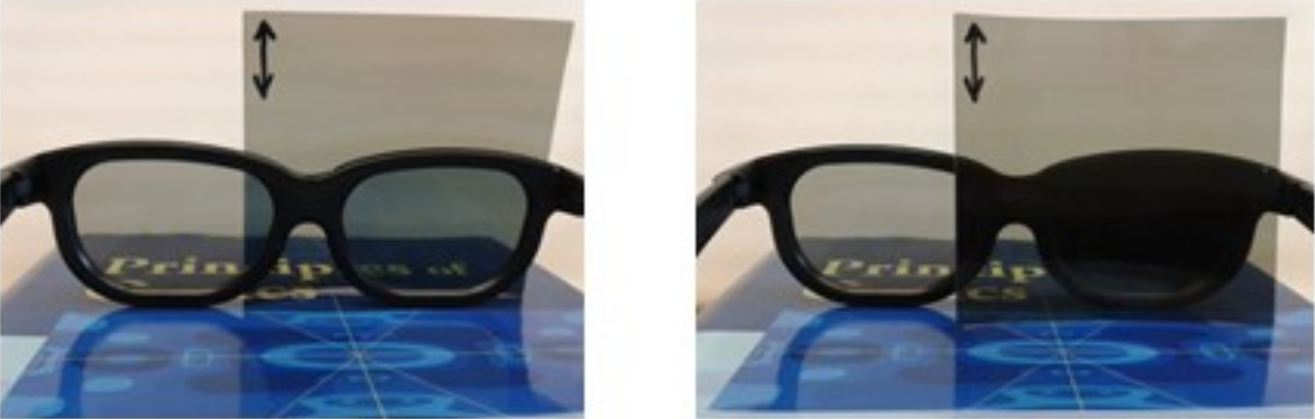
\includegraphics[width=13truecm]{slike/03_VrstniRed.png}
\caption{Učinek vpliva vrstnega reda cirkularnega in linearnega polarizatorja.}
\label{fig:03_VrtsniRed}
\end{figure}

\end{example}

\section{Valovna enačba v prevodni snovi}
Obravnavajmo še homogeno in izotropno snov, ki pa naj bo prevodna, ampak
nenabita ($\varrho_e = 0$). Izhajamo
iz Maxwellovih enačb (enačbe~\ref{eq:Maxwell1}-\ref{eq:Maxwell4}) in zveze:
\beq
\mathbf{j}_e = \sigma \mathbf{E}
\label{eq:03_65}
\eeq
Pri tem smo s $\sigma$ označili električno prevodnost. Tipična vrednost
za kovine je $\sigma > 10^6/\si{\ohm\m}$ in za izolatorje 
$\sigma < 10^{-6}/\si{\ohm\m}$. 
Prevodnost snovi moramo upoštevati pri zapisu Amp\`{e}rovega zakona:
\beq
\nabla\times\mathbf{H} =\frac{\partial\mathbf{D}}{\partial t}+\mathbf{j}_e = 
\varepsilon \varepsilon_0 \frac{\partial\mathbf{E}}{\partial t}+\sigma \mathbf{E}.
\label{eq:03_66}
\eeq
Tudi tokrat izhajamo iz Faradayevega zakona in na njem izvedemo operacijo rotorja:
\beq
\nabla \times \left( \nabla \times  \mathbf{E}\right) = -\nabla\times \left(
\frac{\partial \mathbf{B}}{\partial t}\right) = - \mu \mu_0 \frac{\partial }{\partial t}
\left( \nabla \times \mathbf{H}\right).
\label{eq:03_67}
\eeq.
Vstavimo enačbo~(\ref{eq:03_66}) in dobimo:
\beq
\nabla \times \left( \nabla \times  \mathbf{E}\right) =
 -\mu \mu_0 \frac{\partial }{\partial t}
\left( \varepsilon \varepsilon_0 \frac{\partial\mathbf{E}}{\partial t}\right)-
\mu \mu_0 \frac{\partial }{\partial t}\left(\sigma \mathbf{E} \right).
\label{eq:03_671}
\eeq
Upoštevamo še enačbo~(\ref{eq:03_02}) in dobimo zvezo:
\boxeq{eq:telegrafska}{
\nabla^2\mathbf{E} =  \mu \mu_0\varepsilon \varepsilon_0 \frac{\partial^2\mathbf{E}}{\partial t^2}
+ \mu \mu_0 \sigma \frac{\partial \mathbf{E}}{\partial t}.
}
Zapisano enačbo imenujemo telegrafska enačba. Povsem analogno lahko izpeljemo tudi telegrafsko enačbo
za gostoto magnetnega polja $\mathbf{B}$.

Ker v telegrafski enačbi med drugim nastopa tudi prvi odvod po času, po analogiji z mehanskimi
sistemi pričakujemo, da se valovanje v snovi duši oziroma slabi (atenuira). 
Rešitev zato iščemo v obliki ravnega vala:
\beq
\mathbf{E}(\mathbf{r},t) = \mathbf{E}_0 e^{i\mathbf{k}\cdot \mathbf{r} - i\omega t + i\delta},
\label{eq:03_68}
\eeq
pri čemer dopuščamo možnost kompleksnega valovnega vektorja, katerega imaginarni del
bo opisoval pojemanje amplitude. Ko nastavek (enačba~\ref{eq:03_68})
vstavimo v telegrafsko enačbo (enačba~\ref{eq:telegrafska}), dobimo:
\beq
-k^2 \mathbf{E} = \mu \mu_0\varepsilon \varepsilon_0 \left (-\omega^2 \mathbf{E}\right)
+ \mu \mu_0 \sigma \left(-i \omega\right)\mathbf{E}.
\label{eq:03_69}
\eeq
Sledi:
\beq
k^2 = \mu \mu_0\varepsilon \varepsilon_0 \omega^2 + i \mu \mu_0 \sigma\omega = 
\frac{\omega^2}{c_0^2} \varepsilon \mu  + i \frac{\omega^2}{c_0^2}\frac{\sigma \mu}{\varepsilon_0\omega}.
\label{eq:03_70}
\eeq
Vstavimo valovno število v vakuumu $k_0 = \omega/c_0$ in dobimo:
\beq
k^2 = k_0^2 \left( \varepsilon \mu + i \frac{\sigma \mu}{\varepsilon_0\omega} 
\right)\!\!.
\label{eq:03_71}
\eeq
Vpeljemo kompleksni lomni količnik $\mathcal{N}$, tako da velja:
\boxeq{eq:nkompleks}{
k = k_0 \mathcal{N},
}
pri čemer je:
\boxeq{eq:nkompleks2}{
\mathcal{N}^2 = \varepsilon \mu + i \frac{\sigma \mu}{\varepsilon_0\omega}.
}
Kompleksni lomni količnik $\mathcal{N}$ zapišemo kot vsoto realnega in imaginarnega
dela:
\beq
\mathcal{N}^2 = (n'+in'')^2 = n'^2 -n''^2 + 2i n'n''.
\label{eq:03_72}
\eeq
Izračunajmo realni $n'$ in imaginarni del $n''$ kompleksnega lomnega 
količnika. Označimo realni del $\mathcal{N}^2$ (enačba~\ref{eq:nkompleks2})
z $x = \varepsilon \mu$ in imaginarni del z $y = \sigma \mu/\varepsilon_0\omega$.  
Rešujemo torej:
\beq
x + iy = n'^2 -n''^2 + 2i n'n''.
\label{eq:03_72a}
\eeq
Ločimo realni del:
\beq
x = n'^2 -n''^2
\label{eq:03_73}
\eeq
in imaginarni del:
\beq
y = 2n'n''.
\label{eq:03_74}
\eeq
Izrazimo $n''$ iz druge enačbe in ga vstavimo v prvo. Dobimo kvadratno enačbo:
\beq
n'^2-(y/2n')^2 = x
\label{eq:03_75}
\eeq
z rešitvijo:
\beq
n'^2 = \left(x + \sqrt{x^2+y^2}\right)/2.
\label{eq:03_76}
\eeq
Pri tem smo se omejili na rešitev s pozitivnim predznakom, saj je negativen predznak
za navadne snovi nesmiseln. Iz enačbe~(\ref{eq:03_73}) izračunamo še imaginarni del, 
ki je enak:
\beq
n''^2 = \left(-x + \sqrt{x^2+y^2}\right)/2.
\label{eq:03_77}
\eeq
Vstavimo izraza za $x$ in $y$ in dobimo:
\beq
n'^2 = \frac{1}{2}\left(\varepsilon \mu + \sqrt{(\varepsilon \mu)^2 + 
\left(\frac{\sigma \mu}{\varepsilon_0\omega}\right)^2}\right)
\label{eq:03_78}
\eeq
in
\beq
n''^2 = \frac{1}{2}\left(-\varepsilon \mu + \sqrt{(\varepsilon \mu)^2 + 
\left(\frac{\sigma \mu}{\varepsilon_0\omega}\right)^2}\right)\!\!.
\label{eq:03_79}
\eeq
Pogosto nas zanimajo nemagnetne snovi, v katerih je $\mu=1$.
Kvadrat realnega dela lomnega količnika je potem:
\beq
n'^2 = \frac{1}{2}\left(\varepsilon + \sqrt{\varepsilon^2 + 
\left(\frac{\sigma}{\varepsilon_0\omega}\right)^2}\right)\!\!,
\label{eq:03_80}
\eeq
imaginarnega dela pa:
\beq
n''^2 = \frac{1}{2}\left(-\varepsilon + \sqrt{\varepsilon^2 + 
\left(\frac{\sigma}{\varepsilon_0\omega}\right)^2}\right)\!\!.
\label{eq:03_81}
\eeq
Vstavimo zdaj izračunani lomni količnik v nastavek za jakost električnega polja 
(enačba~\ref{eq:03_68}) in poglejmo
primer, ko je $\mathbf{k} \parallel z$. Dobimo:
\beq
\mathbf{E} = \mathbf{E}_0 e^{ik_0\mathcal{N}z - i\omega t + i\delta} = 
\mathbf{E}_0 e^{ik_0 n'z - i\omega t + i\delta} \cdot e^{-k_0n''z}.
\label{eq:03_82}
\eeq
Zadnji člen opisuje eksponentno pojemanje amplitude polja z globino $z$ in ga pogosto
pišemo kot $\exp(-\kappa z)$, pri čemer je $\kappa = k_0 n''$.

V kovinah je prevodnost zelo velika in velja:
\beq
\frac{\sigma}{\omega\varepsilon_0} \gg \varepsilon.
\label{eq:03_83}
\eeq
Potem lahko imaginarni del lomnega količnika zapišemo kot:
\beq
n'' \approx \sqrt{\frac{\sigma}{2 \omega \varepsilon_0}}.
\label{eq:03_84}
\eeq
Koeficient pojemanja oziroma slabljenja je:
\beq
\kappa = k_0 n'' = \frac{\omega}{c_0} \sqrt{\frac{\sigma}{2 \omega \varepsilon_0}} = \sqrt{\frac{\mu_0 \omega \sigma}{2}}.
\label{eq:03_85}
\eeq
Nazornejše je vpeljati vdorno globino:
\beq
d = \kappa^{-1} = \sqrt{\frac{2}{\mu_0 \omega \sigma}}.
\label{eq:03_86}
\eeq
V kovinah je zaradi velike prevodnosti vdorna globina zelo majhna. Večina elektromagnetnega
valovanja oziroma izmeničnega toka zato teče po površini snovi. Ta pojav poznamo pod imenom
kožni pojav.

\begin{example}{\bf Vdorna globina v bakru.}
Specifična upornost bakra je $\xi = 0,017~\si{\ohm \milli\metre^2/\metre}$ in 
prevodnost $\sigma = 1/\xi = 0,7 \times 10^8/\si{\ohm\metre}$. 
Vdorna globina je odvisna od frekvence, zato izračunajmo nekaj primerov: 
\begin{center}
\begin{tabular}{|c|c|}
\hline
$\nu~[\si{Hz}]$ & $d~[\si{nm}]$\\ \hline
50 & $\approx 10~\si{mm}$\\ \hline
$10^6$ & $\approx 60~\si{\micro\metre}$\\ \hline
$10^9$ & $\approx 0,6~\si{\micro\metre}$\\ \hline
$10^{16}$ & $\approx 0,6~\si{\nano\metre}$\\ \hline
\end{tabular}
\end{center}

Vdorna globina za vidno svetlobo je v bakru torej manjša od nanometra. 
To predstavlja velik problem pri izdelavi prozornih elektrod, 
ki jih potrebujemo na primer za izdelavo sončnih celic
ali tekočekristalnih zaslonov. Zato za ta namen navadno uporabljamo
kovine z razmeroma majhno prevodnostjo (npr. indijev 
kositrov oksid, ITO), pri katerih je dovoljena debelina
plasti, ki jo nanesemo na steklo, razmeroma velika, tipično 
okoli $100~\si{nm}$. 
\end{example}
